% Same toy graph, three models: fully connected, masked BINN, GNN.
% Build: pdflatex binn-gnn.tex && pdftocairo -png -r 300 -transp -singlefile binn-gnn.pdf binn-gnn
\documentclass[tikz,border=4pt]{standalone}
\usepackage[default]{sourcesanspro}
\usepackage[T1]{fontenc}
\usetikzlibrary{arrows.meta}

\definecolor{genome}{HTML}{8E6BBF}
\definecolor{rna}{HTML}{2E9E6E}
\definecolor{gene}{HTML}{9CC3E6}
\definecolor{pw}{HTML}{2A78D6}
\definecolor{root}{HTML}{1C3D6E}
\definecolor{anon}{HTML}{B5B5B5}
\definecolor{edge}{HTML}{8C8C8C}
\definecolor{txt}{HTML}{1C3D6E}
\definecolor{hl}{HTML}{EB6834}

\tikzset{
  n/.style={circle, draw=white, line width=0.8pt, minimum size=14pt, inner sep=0pt},
  omic/.style={rectangle, minimum size=7pt, inner sep=0pt, draw=white, line width=0.5pt},
  e/.style={draw=edge, line width=0.9pt},
  ttl/.style={font=\bfseries\Large, text=txt, anchor=base},
  sub/.style={font=\large, text=edge!80!black, anchor=north, align=center},
}

% coordinates shared by all panels (relative to the panel's scope)
\newcommand{\coords}{
  \foreach \i in {1,...,4} {
    \coordinate (g\i) at ({(\i-2.5)*1.0}, 0);
    \coordinate (a\i) at ({(\i-2.5)*1.0-0.16}, -0.85);   % genome input
    \coordinate (b\i) at ({(\i-2.5)*1.0+0.16}, -0.85);   % RNA input
  }
  \coordinate (p1) at (-0.75, 1.7); \coordinate (p2) at (0.75, 1.7);
  \coordinate (o) at (0, 3.3);
}
% a node drawn as a short vector of cells
\newcommand{\vecnode}[3]{% position, colour, number of cells
  \foreach \c in {1,...,#3}
    \node[rectangle, minimum width=6pt, minimum height=13pt, inner sep=0pt, fill=#2!\fpeval{100-(\c-1)*25},
          draw=white, line width=0.6pt] at ($(#1)+({(\c-(#3+1)/2)*6pt},0)$) {};
}
\usetikzlibrary{calc}

\begin{document}
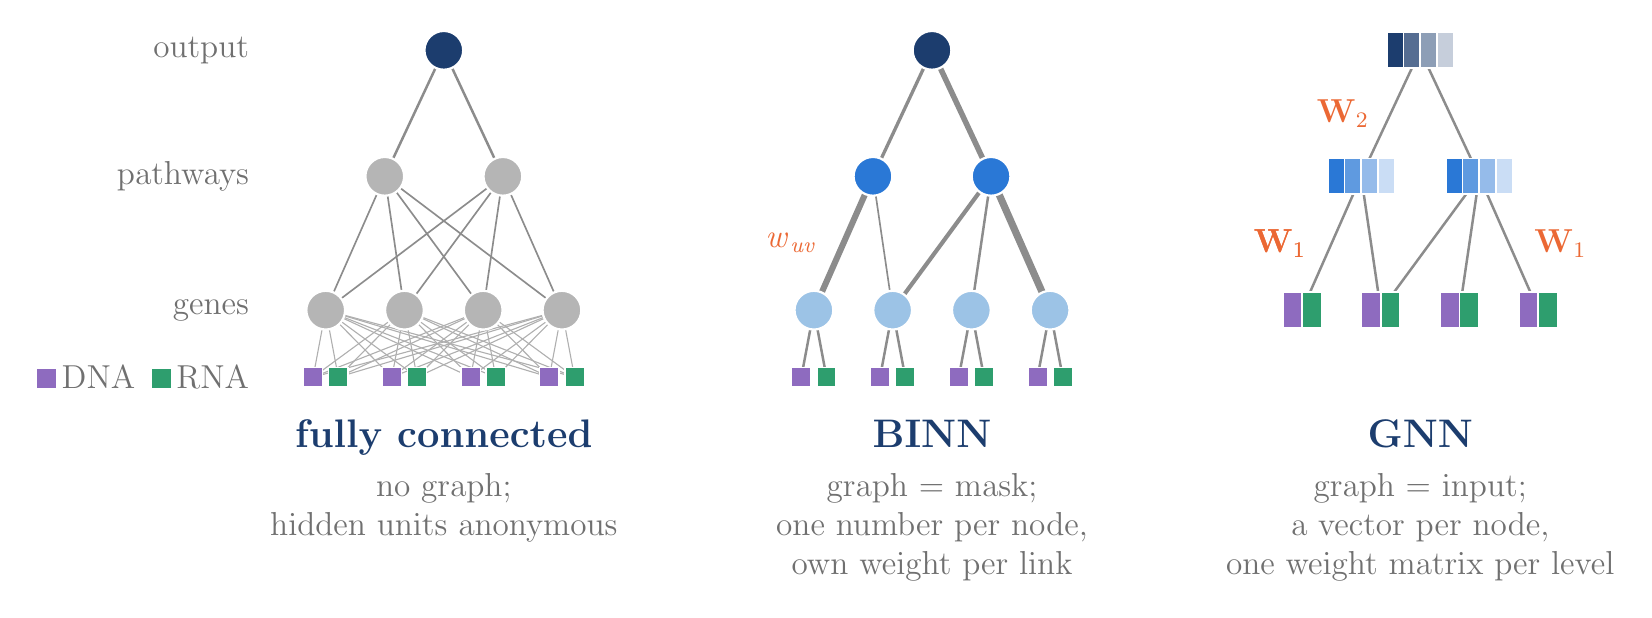
\begin{tikzpicture}

% ---------------- 1. fully connected ----------------
\begin{scope}[xshift=0cm]
  \coords
  \foreach \i in {1,...,4} \foreach \j in {1,...,4} {
    \draw[e, line width=0.4pt, draw=edge!70] (a\i) -- (g\j); \draw[e, line width=0.4pt, draw=edge!70] (b\i) -- (g\j); }
  \foreach \i in {1,...,4} \foreach \j in {1,2} \draw[e, line width=0.6pt] (g\i) -- (p\j);
  \foreach \j in {1,2} \draw[e] (p\j) -- (o);
  \foreach \i in {1,...,4} { \node[omic, fill=genome] at (a\i) {}; \node[omic, fill=rna] at (b\i) {}; }
  \foreach \i in {1,...,4} \node[n, fill=anon] at (g\i) {};
  \foreach \j in {1,2} \node[n, fill=anon] at (p\j) {};
  \node[n, fill=root] at (o) {};
  \node[ttl] at (0,-1.75) {fully connected};
  \node[sub] at (0,-1.95) {no graph;\\hidden units anonymous};
\end{scope}

% ---------------- 2. BINN ----------------
\begin{scope}[xshift=6.2cm]
  \coords
  \foreach \i in {1,...,4} { \draw[e] (a\i) -- (g\i); \draw[e] (b\i) -- (g\i); }
  % one weight per edge: drawn with different widths
  \draw[e, line width=2.2pt] (g1) -- (p1);
  \draw[e, line width=0.6pt] (g2) -- (p1);
  \draw[e, line width=1.5pt] (g2) -- (p2);
  \draw[e, line width=0.9pt] (g3) -- (p2);
  \draw[e, line width=2.6pt] (g4) -- (p2);
  \draw[e, line width=1.2pt] (p1) -- (o);
  \draw[e, line width=2.0pt] (p2) -- (o);
  \foreach \i in {1,...,4} { \node[omic, fill=genome] at (a\i) {}; \node[omic, fill=rna] at (b\i) {}; }
  \foreach \i in {1,...,4} \node[n, fill=gene] at (g\i) {};
  \foreach \j in {1,2} \node[n, fill=pw] at (p\j) {};
  \node[n, fill=root] at (o) {};
  \node[font=\large, text=hl, anchor=east] at ($(g1)!0.5!(p1)+(-0.2,0)$) {\textit{w}\textsubscript{\textit{uv}}};
  \node[ttl] at (0,-1.75) {BINN};
  \node[sub] at (0,-1.95) {graph = mask;\\one number per node,\\own weight per link};
\end{scope}

% ---------------- 3. GNN ----------------
\begin{scope}[xshift=12.4cm]
  \coords
  \draw[e] (g1) -- (p1); \draw[e] (g2) -- (p1); \draw[e] (g2) -- (p2);
  \draw[e] (g3) -- (p2); \draw[e] (g4) -- (p2);
  \draw[e] (p1) -- (o); \draw[e] (p2) -- (o);
  % gene state = its own omics values
  \foreach \i in {1,...,4} {
    \node[rectangle, minimum width=7pt, minimum height=13pt, inner sep=0pt, fill=genome, draw=white, line width=0.6pt] at ($(g\i)+(-3.5pt,0)$) {};
    \node[rectangle, minimum width=7pt, minimum height=13pt, inner sep=0pt, fill=rna, draw=white, line width=0.6pt] at ($(g\i)+(3.5pt,0)$) {};
  }
  \foreach \j in {1,2} \vecnode{p\j}{pw}{4}
  \vecnode{o}{root}{4}
  \node[font=\large, text=hl, anchor=east] at ($(g1)!0.5!(p1)+(-0.2,0)$) {\textbf{W}\textsubscript{1}};
  \node[font=\large, text=hl, anchor=west] at ($(g4)!0.5!(p2)+(0.2,0)$) {\textbf{W}\textsubscript{1}};
  \node[font=\large, text=hl, anchor=east] at ($(p1)!0.5!(o)+(-0.15,0)$) {\textbf{W}\textsubscript{2}};
  \node[ttl] at (0,-1.75) {GNN};
  \node[sub] at (0,-1.95) {graph = input;\\a vector per node,\\one weight matrix per level};
\end{scope}

% legend for the inputs
\node[anchor=east, font=\large, text=edge!80!black, align=right] at (-2.35,-0.85)
  {\textcolor{genome}{\rule{7pt}{7pt}}\,DNA\enspace\textcolor{rna}{\rule{7pt}{7pt}}\,RNA};
\node[anchor=east, font=\large, text=edge!80!black] at (-2.35, 0) {genes};
\node[anchor=east, font=\large, text=edge!80!black] at (-2.35, 1.7) {pathways};
\node[anchor=east, font=\large, text=edge!80!black] at (-2.35, 3.3) {output};
\end{tikzpicture}
\end{document}
